	\subsection{Procedures etc}

	\begin{frame}
	
	
	
	
	\begin{CaixaModelo01}{ATIVIDADE com Procedures etc}
	
Entre no site sitado no slide gráficos, baixo o projeto e execute na maquina

			\begin{figure}
			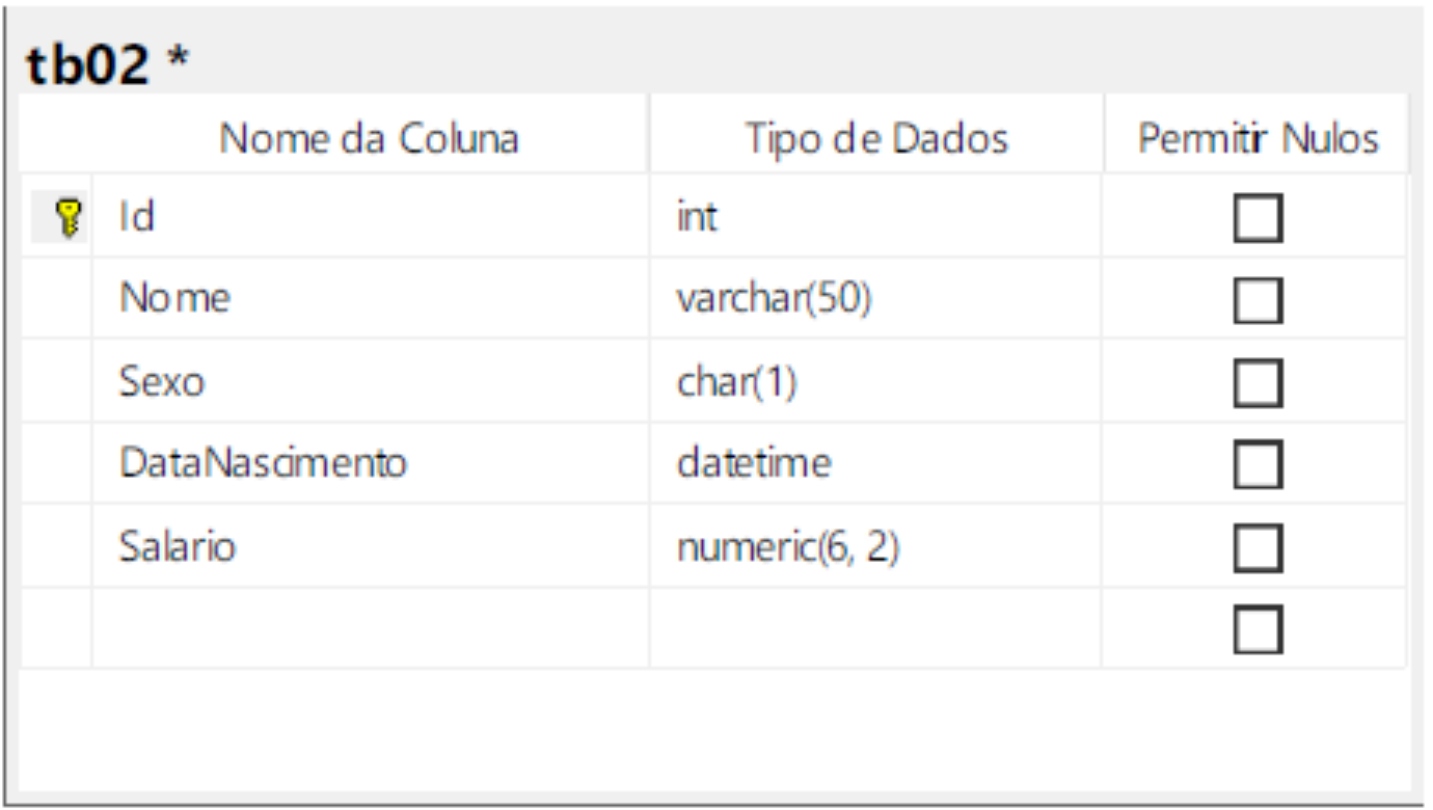
\includegraphics[scale=.6]{./Figuras/Tabela02.png}
			\caption{Tabela de exemplo}
			\label{fig:Tabela02}
			\end{figure}



	\end{CaixaModelo01}

	\end{frame}


	\begin{frame}




\begin{CaixaModelo01}{ATIVIDADE com Procedures etc}
	
	
	\begin{itemize}
		%\item . 
		\item Crie a tabela da figura na base.
		\item Popule a tabela criada com dados de teste.
		\item Crie uma procedure que retorne todos os dados da tabela. 
		\item Crie uma function que retorne todos os dados da tabela. 
		\item Crie uma function que retorne a quantidade de  registros da tabela. 
		\item Crie uma view que retorne todos os dados da tabela. 
		\item Crie uma aplicação que realize a chamada às entidades criadas. 
		\item Crie na aplicação um teste Transacional. 			
	\end{itemize}
	
\end{CaixaModelo01}

\end{frame}